\documentclass[12pt]{article}

\usepackage[utf8]{inputenc}
\usepackage[T1]{fontenc}
\usepackage[brazil]{babel}
\usepackage[margin=2cm]{geometry}
\usepackage{booktabs, float, amsmath,amsthm,amssymb, enumitem, tikz, mdframed, listings, xcolor, graphicx, titling}

\setlength{\droptitle}{-1em}

\renewcommand{\theenumi}{\thesection.\arabic{enumi}}
\renewcommand{\theenumii}{\theenumi.\alph{enumii}}
\newcounter{csol}[enumi]
\renewcommand*{\thecsol}{\theenumi.\alph{csol}}

\lstset{basicstyle=\scriptsize\ttfamily\color{black},
		language=C++,
		frame=single,
		keywordstyle=\color{red},
		stringstyle=\color[rgb]{0,.5,0},
		commentstyle=\color{gray},
		numbers=left,
		numbersep=5pt,
		numberstyle=\tiny\color{gray},
		showspaces=false,
		showstringspaces=false,
		tabsize=4
		}
	
\title{Matemática Concreta - Listas de exercícios}
\author{Helder Mateus dos Reis Matos - 201904940036}
\date{28 de outubro de 2020}

\begin{document}

\maketitle

\textbf{Atenção: } As questões de implementação foram feitas em C++. Passos importantes dos programas são descritos pelas indicações de linhas \verb|[inicial:final]|, com limites inclusivos.

\setcounter{section}{1}
\section*{Atividade aula 1}

\begin{enumerate}
	\item \textbf{Escolha uma linguagem de programação, implemente as funções de recorrência e exiba os seis primeiros termos de cada sequência. Inclua o código fonte das funções na resposta.}
	\begin{enumerate}
		\item $a_1 = 5$ e $a_n = a_{n-1}+3, \forall n > 1$
		\lstinputlisting{../src/1_1a.cpp}

		\item $b_1 = 2$ e $b_n = b_{n-1}^2, \forall n > 1$
		\lstinputlisting{../src/1_1b.cpp}

		\item $c_1 = 0$ e $c_n = 2c_{n-1}+n, \forall n > 1$
		\lstinputlisting{../src/1_1c.cpp}
	\end{enumerate}

	\item \textbf{Escolha uma linguagem de programação e escreva um programa para receber uma sequência numérica e informar se a sequência é um P.A ou não. Caso seja uma P.A, o programa deve informar se a P.A é crescente, constante ou decrescente.}
	\lstinputlisting{../src/1_2.cpp}
	\verb|[3:10]| - A função \verb|checar_pa| recebe um array contendo a sequência, a razão entre os dois primeiros elementos e o seu tamanho $n$. Se a diferença entre um termo da sequência e o seu anterior for diferente da razão, a sequência não é P.A. Caso a razão se mantenha constante pra cada par de elementos, a sequência é P.A. \\
	\verb|[12:29]| - \verb|categorizar_pa| recebe apenas a sequência e seu tamanho. Ao calcular a razão entre o segundo e primeiro termo, é chamada a função \verb|checar_pa|, que dependendo do seu retorno e do valor da razão, classifica a sequência em "não P.A.", P.A. crescente, P.A. decrescente ou P.A. constante.
	
	\item \textbf{Sabendo que o primeiro termo é igual a 3 e a razão é igual a 5, calcule o 17 o termo de uma P.A.}\\
	O enésimo termo de uma P.A., onde o primeiro termo é $a_1$ e a razão é $r$, é dado por:
	$$ a_n = a_1 + (n-1)r $$
	Tomando $a_1 = 3$, $r=5$ e $n=17$, temos:
	$$ a_{17} = 3 + (17-1)5 $$
	$$ a_{17} = 3 + 16 \cdot 5 $$
	$$ a_{17} = 3 + 80 $$
	$$ a_{17} = 83 $$
	
	\item \textbf{Sabendo que o primeiro termo é igual a -8 e o vigésimo igual a 30, calcule a razão da P.A.}\\
	Partindo da definição do enésimo termo de uma P.A., a razão pode ser encontrada por:
	$$ a_n = a_1 + (n-1)r $$
	$$ (n-1)r = a_n - a_1 $$
	$$ r = \frac{a_n - a_1}{n-1} $$
	De posse de $a_1 = -8$ e $a_n = a_{20} = 30$, a razão desta P.A. é:
	$$ r = \frac{30 - (-8)}{20-1} $$
	$$ r = \frac{38}{19} $$
	$$ r = 2 $$
	
	\pagebreak
	\item \textbf{Escolha uma linguagem de programação e escreva um programa para receber os extremos de uma P.A, o valor de K e calcule a interpolação dessa P.A.}
	\lstinputlisting{../src/1_5.cpp}
	\verb|[3:10]| - O procedimento \verb|interpor_pa| recebe uma sequência vazia, os extremos da P.A. e a quantidade $k$ de elementos entre os extremos. De posse da razão, cada elemento da P.A. é inserido na sequência, começando do primeiro até o último, conforme o valor da razão.\\
	\verb|[23:33]| - Como o tamanho da sequência ($k+2$) depende da entrada e não é mais alterado, optou-se pela alocação dinâmica do array, ao invés de estruturas mais sofisticadas.
		
	\item \textbf{Calcule a P.A em que a soma dos n primeiros termos é igual a $n^2 + 2n$.}\\
	Conhecendo a expressão da soma dos $n$ termos, podemos encontrar a soma $S_1$ do primeiro termo, que nada mais é do que o primeiro termo:
	$$ S_n = n^2 + 2n$$
	$$ S_1 = 1^2 + 2 \cdot 1 = 3 \quad \therefore \quad a_1 = 3 $$
	Encontrando a soma $S_2$ dos dois primeiros termos, podemos encontrar o segundo termo, pois ele é a diferença entre $S_2$ e $S_1$. Para os demais termos, o procedimento é semelhante:
	$$ S_2 = 2^2 + 2 \cdot 2 = 8 \quad \therefore \quad a_2 = S_2 - S_1 = 8 - 3 = 5 $$
	$$ S_3 = 3^2 + 2 \cdot 3 = 15 \quad \therefore \quad a_3 = S_3 - S_2 = 15 - 8 = 7 $$
	$$ S_4 = 4^2 + 2 \cdot 4 = 24 \quad \therefore \quad a_4 = S_4 - S_3 = 24 - 15 = 9 $$
	$$ S_5 = 5^2 + 2 \cdot 5 = 35 \quad \therefore \quad a_5 = S_5 - S_4 = 35 - 22 = 11 $$
	Pode-se verificar a formação de uma progressão aritmética de razão $2$, portanto os demais elementos sempre aumentarão com esta razão.\\
	Generalizando, $a_n = S_n - S_{n-1} = (n^2 + 2n) - ((n-1)^2 + 2(n-1))$, para $S_1 = a_1 = 3$.
	
	\item \textbf{Escolha uma linguagem de programação e escreva um programa para receber uma sequência numérica e informar se a sequência é um P.G ou não. Caso seja uma P.G, o programa deve informar se a P.G é crescente, constante, decrescente, alternante ou estacionária.}
	\lstinputlisting{../src/1_7.cpp}
	\verb|[6:8]| - Excepcionalmente nessa solução é possível fazer a entrada de sequência de números reais fracionários, e.g. $1/3$. Para solucionar o problema de precisão na representação de pontos flutuantes foi criada a função \verb|chao| que arredonda um número real para baixo, com precisão de 6 casas decimais.\\
	\verb|[10:35]| - Para a entrada de números reais fracionários, foi criada a função \verb|parse_stof| que converte strings em valores numéricos, além de verificar se há sinal de divisão \verb|'/'| dentre os números da sequência inserida. Caso exista, é efetuada a divisão entre o numerador e o denominador. Desse modo, é possível representar com mais exatidão dízimas periódicas.\\
	\verb|[37:46]| - Não há função nativa em C++ para dividir uma string por caractere, como em outras linguagens. A função \verb|split| foi criada com esse intuito, dividindo a stream de strings inserida pelo usuário em strings divididas por espaços simples. Em seguida a função \verb|parse_stof| é chamada para a conversão das strings em floats.\\
	\verb|[48:55]| - É retornado de \verb|checar_pg| um booleano indicando se a sequência informada é uma P.G., baseada na razão $q$ entre os dois primeiros números.\\
	\verb|[57:81]| - A P.G. é classificada de acordo com o valor de $q$, e, quando necessário, do sinal dos termos da sequência. Caso $q > 1$ para termos positivos ou $0 < q < 1$ para termos negativos, a P.G. é crescente. Caso $0 < q < 1$ para termos negativos ou $q > 1$ para termos positivos, a P.G. é decrescente. Se $q = 1$ para termos não nulos, a P.G. é constante. Se $q < 0$, os termos alternam o sinal. Para $q = 0$, a P.G. é estacionária.
	
	\item \textbf{Escolha uma linguagem de programação e escreva um programa para receber os extremos de uma P.G, o valor de K e calcule a interpolação dessa P.G.}
	\lstinputlisting{../src/1_8.cpp}
	\verb|[4:12]| - \verb|interpor_pa| recebe a sequência vazia, o extremo inferior $a_1$, o extremo superior $a_ n$ e o valor de $k$ termos intermediários. A razão entre elementos consecutivos $q = \sqrt[k+1]{\frac{a_n}{a_1}}$ é usada para incrementar geometricamente o valor de $a_1$ a cada iteração no array que armazena a sequência.
	
	\item \textbf{Escolha uma linguagem de programação e escreva um programa para receber uma sequência numérica. Se a sequência numérica for uma P.G, informe a produto e a soma dos termos dessa P.G. Caso contrário, informe que a sequência não é uma P.G.}
	\lstinputlisting{../src/1_9.cpp}
	\verb|[5:7]| - Desta vez não se fará o uso de entradas em forma de fração, mas manteve-se a função de arrendondamento para baixo, pois os resultados das divisões a seguir podem ser fracionários e não serem representados de forma precisa, ocasionando inconsistência ao compará-los com outros números fracionários.\\
	\verb|[9:16]| - \verb|checar_pg| verifica se a razão entre cada elemento da sequência e seu antecessor é igual à razão entre os dois primeiros.
	\verb|[18:33]| - O procedimento \verb|soma_produto_pg| recebe a sequência e seu tamanho e verifica se é uma P.G. Se for, ocorre a aplicação da soma da P.G, $S_{P.G.} = \frac{a_1q^n-a_ 1}{q-1}$, e do produto da P.G., $P_{P.G.} = a_1^n\cdot q^{\frac{n(n-1)}{2}}$. Em seguida, os resultados são apresentados.

	\item \textbf{Determine o valor de $n$ tal que $\sum_{i=3}^n 2^i = 4088$}\\
	Para encontrar a soma de $i=3$ até $n$, basta notar que a soma de $i=1$ até $n$ pode ser representada da seguinte forma:
	$$\sum_{i=1}^{n} 2^i = \sum_{i=1}^{2} 2^i + \sum_{i=3}^{n} 2^i$$
	O lado esquerdo representa a soma de uma progressão geométrica.
	$$\frac{a_1q^n-a_1}{q-1} = \sum_{i=1}^{2} 2^i + \sum_{i=3}^{n} 2^i$$
	Tomando $a_1 = 2^1 = 2$ e $q = 2$, e substituindo os valores que já conhecemos do lado direito obtemos:
	$$\frac{2\cdot 2^n-2}{2-1} = (2+4) + 4088$$
	$$2\cdot 2^n-2 = 6 + 4088$$
	$$2\cdot2^n = 4094+2$$
	$$2^n = \frac{4096}{2}$$
	$$2^n = 2048$$
	$$2^n = 2^{11}$$
	$$n = 11$$
	
\end{enumerate}
\pagebreak

\setcounter{section}{3}
\section*{Atividade aula 3}

\begin{enumerate}
	\item \textbf{Escolha uma linguagem de programação e escreva um programa que receba	uma sequência digitada pelo usuário e exiba a subsequência de números ímpares.}
	\lstinputlisting{../src/3_1.cpp}
	\verb|[4:12]| - Nas soluções da lista 3 foi utilizada a classe de objetos do C++ \verb|std::vector|, pela facilidade e flexibilidade ao armazenar, inserir e referenciar elementos. \verb|subseq_impar| recebe uma sequência e retorna a subsequência de números ímpares.
	
	\pagebreak
	\item \textbf{Escolha uma linguagem de programação e escreva um programa que receba	uma sequência digitada pelo usuário e exiba a subsequência de números primos.}
	\lstinputlisting{../src/3_2.cpp}
	\verb|[5:13]| - \verb|primacidade| retorna um booleano indicando a primacidade de um número.\\
	\verb|[15:21]| - \verb|subseq_primos| retorna a subsequência de números primos, a partir da sequência de entrada.
	
	\pagebreak
	\item \textbf{Escolha uma linguagem de programação e escreva um programa que receba	duas sequências A e B digitada pelo usuário e exiba a concatenação BA.}
	\lstinputlisting{../src/3_3.cpp}
	\verb|[4:11]| - \verb|concatenar| faz a inserção dos vetores \verb|vec1| e \verb|vec2| em um vetor vazio \verb|concatenacao|. Note que \verb|vec1| é sempre inserido antes de \verb|vec2|, logo a ordem dos vetores na chamada da função importa (linha \verb|[35]|).
	
	\pagebreak
	\item \textbf{Escolha uma linguagem de programação e escreva um programa que receba	uma sequência, os índices $a$ e $b$ digitados pelo usuário, e exiba o segmento com os extremos $x_a$ e $x_b$. Considere que sempre $a \leq b$.}
	\lstinputlisting{../src/3_4.cpp}
	\verb|[4:12]| - \verb|segmentar| recebe a sequência de entrada e os limites do segmento. O segmento vazio é declarado com um tamanho $b-a+1$. São declarados dois iteratores, que apontam para início (iterador \verb|begin()|, apontando para o primeiro elemento da entrada + a) e fim (iterador \verb|begin()|, apontando para o primeiro elemento da entrada, + b + 1) do segmento, respectivamente. Assim, os elementos que estão entre os limites indicados pelos iteradores são copiados para o segmento vazio.
	
	\pagebreak
	\item \textbf{Escolha uma linguagem de programação e escreva um programa que receba	uma sequência, o valor $k$ digitado pelo usuário, e exiba o prefixo de comprimento $k$.}
	\lstinputlisting{../src/3_5.cpp}
	\verb|[4:12]| - Semelhante à solução anterior, os elementos que estão entre os limites apontados pelos iteradores de início (iterador \verb|begin()|, apontando para o primeiro elemento da entrada) e fim (iterador \verb|begin()|, apontando para o primeiro elemento da entrada + k) são copiados para um vetor \verb|prefixo| de tamanho $k$.
	
	\pagebreak
	\item \textbf{Escolha uma linguagem de programação e escreva um programa que receba	uma sequência, o valor $k$ digitado pelo usuário, e exiba o sufixo de comprimento $k$.}
	\lstinputlisting{../src/3_6.cpp}
	\verb|[4:12]| - Para encontrar o início do sufixo, o iterador \verb|begin()| é acrescido da diferença entre o tamanho da entrada pelo tamanho do sufixo. O iterador \verb|end()| aponta para o último elemento da sequência. Assim, os elementos entre os dois iteradores são copiados para o vetor \verb|sufixo|.
	
\end{enumerate}
\pagebreak

\setcounter{section}{5}
\section*{Atividade aula 5}

\begin{enumerate}
	\item \textbf{Utilizando as propriedades do somatório, mostre que:}
	$$\sum_{k=1}^{n}(x_{k+1}-x_k) = x_{n+1}-x_1$$
	Através da propriedade associativa temos:
	$$\sum_{k=1}^{n}(x_{k+1}-x_k) = \sum_{k=1}^{n}x_{k+1} - \sum_{k=1}^{n}x_k$$
	Podemos incrementar os índices dos limites do primeiro somatório, ao decrementar na mesma proporção o índice da fórmula do mesmo.
	$$\sum_{k=1}^{n}(x_{k+1}-x_k) = \sum_{k=2}^{n+1}x_{k} - \sum_{k=1}^{n}x_k$$
	Podemos retirar as parcelas mais próximas dos extremos de um somatório. Vamos retirar a última parcela do primeiro e a primeira parcela do segundo.
	$$\sum_{k=1}^{n}(x_{k+1}-x_k) = x_{n+1}+\sum_{k=2}^{n}x_{k} - \left(x_1+\sum_{k=2}^{n}x_k\right)$$
	Simplificando, obtemos a relação dada, como se queria demonstrar:
	$$\sum_{k=1}^{n}(x_{k+1}-x_k) = x_{n+1}+\sum_{k=2}^{n}x_{k} - x_1-\sum_{k=2}^{n}x_k$$
	$$\sum_{k=1}^{n}(x_{k+1}-x_k) = x_{n+1} - x_1$$

	\item \textbf{Utilizando as propriedades do somatório, mostre que:}
	$$\sum_{k=1}^{n}k(k+1) = \frac{n(n+1)(n+2)}{3}$$
	Expandindo o somatório original:
	$$\sum_{k=1}^{n}k(k+1) = \sum_{k=1}^{n}k^2 + k$$
	Usando a propriedade associativa:
	$$\sum_{k=1}^{n}k(k+1) = \sum_{k=1}^{n}k^2 + \sum_{k=1}^{n}k$$
	Ambos os somatórios são conhecidos, e ao substituirmos:
	$$\sum_{k=1}^{n}k(k+1) = \frac{n(n+1)(2n+1)}{6} + \frac{n(n+1)}{2}$$
	Simplificando, obtemos a relação dada, como se queria demonstrar:
	$$\sum_{k=1}^{n}k(k+1) = \frac{(n^2+n)(2n+1)}{6} + \frac{n^2+n}{2}$$
	$$\sum_{k=1}^{n}k(k+1) = \frac{2n^3+n^2+2n^2+n}{6} + \frac{n^2+n}{2}$$
	$$\sum_{k=1}^{n}k(k+1) = \frac{2n^3+n^2+2n^2+n + 3n^2+3n}{6}$$
	$$\sum_{k=1}^{n}k(k+1) = \frac{2n^3+6n^2+4n}{6}$$
	$$\sum_{k=1}^{n}k(k+1) = \frac{n^3+3n^2+2n}{3}$$
	$$\sum_{k=1}^{n}k(k+1) = \frac{n(n^2+3n+2)}{3}$$
	$$\sum_{k=1}^{n}k(k+1) = \frac{n(n+1)(n+2)}{3}$$
	
	\item \textbf{Utilizando as propriedades do somatório, mostre que:}
	$$\sum_{k=0}^{n-1}2^k = 2^n-1$$
	O somatório original é uma parcela de um somatório já conhecido, $\sum_{k=0}^{n}2^k$. Note que o somatório dado compreende as somas entre $k=0$ e $k=n-1$, restando apenas a adição da última parcela, $2^n$, para obtermos o somatório de $2^k$, mencionado acima.
	$$\sum_{k=0}^{n-1}2^k = \left(\sum_{k=0}^{n}2^k\right) - 2^n$$
	Substituindo $\sum_{k=0}^{n}2^k = 2^{n+1}-1$:
	$$\sum_{k=0}^{n-1}2^k = 2^{n+1}-1 - 2^n$$
	Simplificando, obtemos a relação dada, como se queria demonstrar:
	$$\sum_{k=0}^{n-1}2^k = (2^{n}2^1)-1 - 2^n$$
	$$\sum_{k=0}^{n-1}2^k = 2^n(2-1)-1$$
	$$\sum_{k=0}^{n-1}2^k = 2^n-1$$
	
	\item \textbf{Utilizando as propriedades do somatório, mostre que:}
	$$\sum_{k=1}^{n}k2^{k-1} = 2^n(n-1)+1$$
	\textbf{Observe que: $2^{k-1}=2^k-2^{k-1}$}\\
	Analisando a expressão do somatório, é possível observar que a mesma é a derivada de outro somatório conhecido, $\sum_{k=0}^{n} x^k = \frac{x^{n+1}-1}{x-1}$:
	$$\sum_{k=1}^{n}k2^{k-1} = \dfrac{d}{dx} \left(\sum_{k=0}^{n} x^k\right) = \dfrac{d}{dx} \left(\frac{x^{n+1}-1}{x-1}\right)$$
	Tomando apenas as duas últimas igualdades, podemos generalizar essas relações:
	$$\dfrac{d}{dx} \left(\sum_{k=0}^{n} x^k\right) = \dfrac{d}{dx} \left(\frac{x^{n+1}-1}{x-1}\right)$$
	Resolvendo ambas as derivadas, obtemos um expressão geral para qualquer valor de $x$:
	$$\sum_{k=1}^{n}kx^{k-1} = \frac{[(x^{n+1}-1)'(x-1)]-[(x^{n+1}-1)(x-1)']}{(x-1)^2}$$
	$$\sum_{k=1}^{n}kx^{k-1} = \frac{(n+1)x^n(x-1)-(x^{n+1}-1)}{(x-1)^2}$$
	$$\sum_{k=1}^{n}kx^{k-1} = \frac{(n+1)x^n(x-1)-x^{n+1}+1}{(x-1)^2}$$
	Tomando $x=2$, obtemos a relação dada, como se queria demonstrar:
	$$\sum_{k=1}^{n}k2^{k-1} = \frac{(n+1)2^n(2-1)-2^{n+1}+1}{(2-1)^2}$$
	$$\sum_{k=1}^{n}k2^{k-1} = 2^n(n+1)-2^{n+1}+1$$
	$$\sum_{k=1}^{n}k2^{k-1} = 2^n(n+1)-2^n2^1+1$$
	$$\sum_{k=1}^{n}k2^{k-1} = 2^n(n+1-2)+1$$
	$$\sum_{k=1}^{n}k2^{k-1} = 2^n(n-1)+1$$
	
	\item \textbf{Utilizando as propriedades do somatório, mostre que:}
	$$\sum_{k=1}^{100}(3-2k)^2 = 1293700$$
	Expandindo a fórmula do somatório:
	$$\sum_{k=1}^{100}(3-2k)^2 = \sum_{k=1}^{100}4k^2-12k+9$$
	Pela propriedade da distributividade:
	$$\sum_{k=1}^{100}(3-2k)^2 = \sum_{k=1}^{100}4k^2-\sum_{k=1}^{100}12k+\sum_{k=1}^{100}9$$
	Retirando as constantes dos somatórios:
	$$\sum_{k=1}^{100}(3-2k)^2 = \left(4\sum_{k=1}^{100}k^2\right) - \left(12\sum_{k=1}^{100}k\right) + \left(9\sum_{k=1}^{100}\right)$$
	Substituindo os somatórios já conhecidos:
	$$\sum_{k=1}^{100}(3-2k)^2 = \left(4\frac{n(n+1)(2n+1)}{6}\right) - \left(12\frac{n(n+1)}{2}\right) + \left(9\cdot n\right)$$
	Substituindo $n=100$, obtemos a relação dada, como se queria demonstrar:
	$$\sum_{k=1}^{100}(3-2k)^2 = \left(4\frac{100(100+1)(2\cdot 100+1)}{6}\right) - \left(12\frac{100(100+1)}{2}\right) + \left(9\cdot 100\right)$$
	$$\sum_{k=1}^{100}(3-2k)^2 = (4\cdot 338350) - (12 \cdot 5050) + (9\cdot 100)$$
	$$\sum_{k=1}^{100}(3-2k)^2 = 1353400 - 60600 + 900$$
	$$\sum_{k=1}^{100}(3-2k)^2 = 1293700$$
	
	\pagebreak
	\item \textbf{Utilizando uma linguagem de programação, codifique o seguinte somatório em que $n$, $x_i$ e $y_i$ são valores digitados pelo usuário:}
	$$\sum_{i=1}^{n}x_i y_i$$
	\lstinputlisting{../src/5_6.cpp}
	
	\item \textbf{Utilizando uma linguagem de programação, codifique o seguinte somatório em que $n$ é informado pelo usuário:}
	$$\sum_{i=1}^{n}i$$
	\lstinputlisting{../src/5_7.cpp}

	\item \textbf{Utilizando uma linguagem de programação, codifique o seguinte somatório em que $n$ e $b_i$ são valores digitados pelo usuário:}
	$$\sum_{i=1}^{n}b_i^2$$
	\lstinputlisting{../src/5_8.cpp}
	
	\item \textbf{Utilizando uma linguagem de programação, codifique o seguinte somatório em que $n$ é informado pelo usuário:}
	$$\sum_{i=0}^{n}2^i$$
	\lstinputlisting{../src/5_9.cpp}
	
	\item \textbf{Utilizando uma linguagem de programação, codifique o seguinte somatório em que $n$, $x_i$ e $y_i$ são valores digitados pelo usuário:}
	$$\sum_{i=1}^{n}\frac{1}{x_i}+\frac{1}{y_i}$$
	\lstinputlisting{../src/5_10.cpp}
	
\end{enumerate}
\pagebreak

\setcounter{section}{7}
\section*{Atividade aula 7}

\begin{enumerate}
	\item \textbf{Utilizando uma linguagem de programação, codifique um somatório para somar os valores as posições de cor verde da matriz. Os valores dessa posições devem ser informados pelo usuário.}
	\begin{figure}[H]
		\centering
		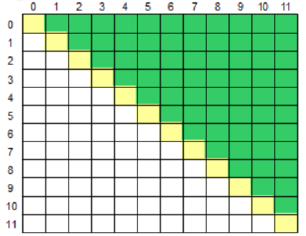
\includegraphics{7_1}
	\end{figure}
	\lstinputlisting{../src/7_1.cpp}
	\verb|[12:24]| - A soma dos valores nas posições verdes (acima da diagonal principal) é acumulada sempre que o índice das linhas for menor que o índice das colunas.

	\pagebreak
	\item \textbf{Utilizando uma linguagem de programação, codifique um somatório para somar os valores as posições de cor verde da matriz. Os valores dessa posições devem ser informados pelo usuário.}
	\begin{figure}[H]
		\centering
		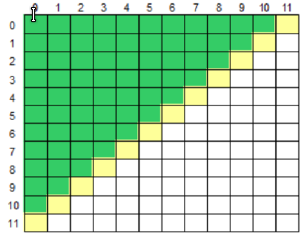
\includegraphics{7_2}
	\end{figure}
	\lstinputlisting{../src/7_2.cpp}
	\verb|[12:24]| - A soma dos valores nas posições verdes (acima da diagonal secundária) é acumulada sempre que a soma do índice das linhas com o índice das colunas for menor que o tamanho da matriz $-1$.
	
	\pagebreak
	\item \textbf{Utilizando uma linguagem de programação, codifique um somatório para somar os valores as posições de cor verde da matriz. Os valores dessa posições devem ser informados pelo usuário.}
	\begin{figure}[H]
		\centering
		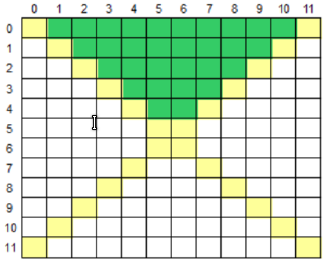
\includegraphics{7_3}
	\end{figure}
	\lstinputlisting{../src/7_3.cpp}
	\verb|[12:24]| - A soma dos valores nas posições verdes (acima de ambas as diagonais) é acumulada sempre que os índices forem parte da interseção entre os valores acima da diagonal principal e acima da diagonal secundária.
	
	\pagebreak
	\item \textbf{Utilizando uma linguagem de programação, codifique um somatório para somar os valores as posições de cor verde da matriz. Os valores dessa posições devem ser informados pelo usuário.}
	\begin{figure}[H]
		\centering
		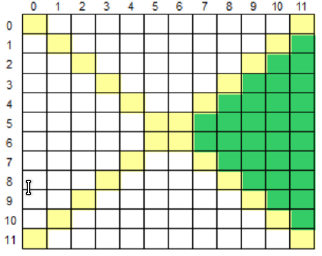
\includegraphics{7_4}
	\end{figure}
	\lstinputlisting{../src/7_4.cpp}
	\verb|[12:24]| - A soma dos valores nas posições verdes (entre ambas as diagonais, pela direita) é acumulada sempre que os índices forem parte da interseção entre os valores acima da diagonal principal e abaixo da diagonal secundária.
	
	\pagebreak
	\item \textbf{Utilizando uma linguagem de programação, codifique um somatório para somar os valores as posições de cor verde da matriz. Os valores dessa posições devem ser informados pelo usuário.}
	\begin{figure}[H]
		\centering
		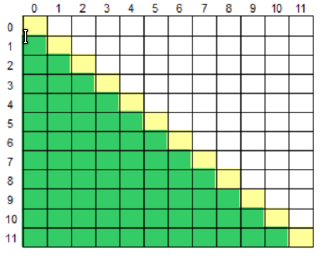
\includegraphics{7_5}
	\end{figure}
	\lstinputlisting{../src/7_5.cpp}
	\verb|[12:24]| - A soma dos valores nas posições verdes (abaixo da diagonal principal) é acumulada sempre que os índices das linhas for maior que o índice das colunas.
	
	\pagebreak
	\item \textbf{Utilizando uma linguagem de programação, codifique um somatório para somar os valores as posições de cor verde da matriz. Os valores dessa posições devem ser informados pelo usuário.}
	\begin{figure}[H]
		\centering
		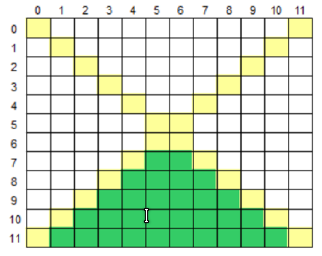
\includegraphics{7_6}
	\end{figure}
	\lstinputlisting{../src/7_6.cpp}
	\verb|[12:24]| - A soma dos valores nas posições verdes (abaixo de ambas as diagonais) é acumulada sempre que os índices forem parte da interseção entre os valores abaixo da diagonal principal e abaixo da diagonal secundária.
	
	\pagebreak
	\item \textbf{Utilizando uma linguagem de programação, codifique um somatório para somar os valores as posições de cor verde da matriz. Os valores dessa posições devem ser informados pelo usuário.}
	\begin{figure}[H]
		\centering
		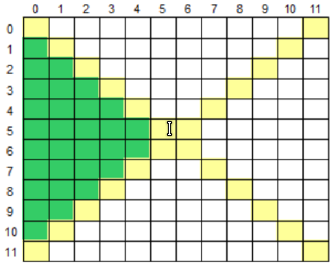
\includegraphics{7_7}
	\end{figure}
	\lstinputlisting{../src/7_7.cpp}
	\verb|[12:24]| - A soma dos valores nas posições verdes (entre ambas as diagonais, pela esquerda) é acumulada sempre que os índices forem parte da interseção entre os valores abaixo da diagonal principal e acima da diagonal secundária.
	
	\pagebreak
	\item \textbf{Utilizando uma linguagem de programação, codifique um somatório para somar os valores as posições de cor verde da matriz. Os valores dessa posições devem ser informados pelo usuário.}
	\begin{figure}[H]
		\centering
		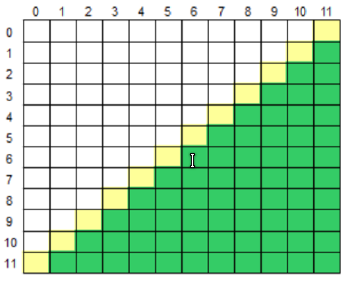
\includegraphics{7_8}
	\end{figure}
	\lstinputlisting{../src/7_8.cpp}
	\verb|[12:24]| - A soma dos valores nas posições verdes (abaixo da diagonal secundária) é acumulada sempre que a soma do índice das linhas com o índice das colunas for maior que o tamanho da matriz $-1$.
	
\end{enumerate}

\end{document}
